\chapter{Измерение качества тематических иерархий}
В обзоре литературы были рассмотрены метрики качества для отдельных тем в тематических моделях. Принятые метрики согласованы с человеческими оценками того, является тема хорошей или плохой.

Тематические иерархии состоят из тем и связей между темами соседних уровней иерархии. Тогда для оценки качества иерархии необходимо измерять не только качество отдельных тем, но и качество отношений "родитель-ребенок"\ в иерархии. В этой работе предлагается несколько метрик качества для ребер иерархии, которые аппроксимируют мнение асессоров о наличии или отсутствии связи между темами.  

\section{Метрики качества ребер иерархии}
\subsection{Метрики на основе лингвистической близости}
 Используем такой же вид метрики качества, что используется при оценке качества отдельных тем, для учета синтагматической или парадигматической родственности топ-токенов темы-родителя и темы-ребенка \cite{Schutze1993}:

$$\mathrm{S}(a, t) = \dfrac{1}{n^2}\sum\limits_{i=1}^{n}\sum\limits_{j=1}^n f(w_i^{(a)}, w_j^{(t)}),$$

Здесь $w_i^{(s)}$ -- это $i$-ый топ-токен некоторой темы $s$. Тема $a \in A$ -- тема $l$-го (родительского) уровня $t\in T$ -- тема $(l+1)$-го (дочернего) уровня, $f(\cdot, \cdot)$ -- мера близости токенов.

Используя ту же меру близости, основанную на совстречаемости токенов, что используется в классической когерентности из \cite{Mimno2011}, получим оценку сходства между темами 

$$\mathrm{S}_{coh}(a, t) = \dfrac{1}{n^2}\sum\limits_{i=1}^n \sum\limits_{j=1}^n \ln \dfrac{D(w^{(a)}_i, w^{(t)}_j) + \varepsilon}{D(w^{(t)}_j)}[w_i^{(a)} \neq w_j^{(t)}].$$ 

Здесь $D(w_1, w_2)$ -- количество документов в некотором корпусе, где слова $w_1$ и $w_2$ встретились вместе, а $D(w)$ -- количество документов, в которых встречается токен $w$.

Используя меру близости из \cite{Nikolenko2016}, основанную на векторных представлениях слов с косинусным расстоянием между векторами, получим метрику 

$$\mathrm{S}_{emb}(a, t) = \dfrac{1}{n^2}\sum\limits_{i=1}^n \sum\limits_{j=1}^n \langle v(w^{(a)}_i), v(w^{(t)}_j)\rangle[w_i^{(a)} \neq w_j^{(t)}],$$ 

где $v(w^{(t)})$ -- вектор, соотвествующий топ-токену $w^{(t)}$ темы $t$ в пространстве word embedding.

\subsection{Метрики на основе вероятностной близости}
В тематической иерархии каждая тема представлена вероятностями токенов в ней, значит можно сравнивать родительские и дочерние темы как вероятностные распределения. Используя две стандартные меры расстояния между распределениями -- расстояние Хеллингера и дивиргенцию Кульбака-Лейблера -- получим следующие метрики:

$$ \mathrm{S}_{Hell}(a, t) = \dfrac{1}{\sqrt{2}} \| \sqrt{p(w|a)} - \sqrt{p(w|t)}\|_2,$$

$$\mathrm{S}_{KL}(a, t) = -D_{KL}(p(w|a)\|p(w|t)).$$

\section{Асессорская разметка ребер иерархии}
Следуя логике, используемой для проверки предлагаемых метрик качества в \cite{Mimno2011, Nikolenko2016}, был проведен асессорский эксперимент, чтобы собрать человеческие оценки качества ребер иерархии.

\subsection{Описанные данных и моделей}
Чтобы собрать пары "родитель-ребенок"\ для аннотации людьми, были обучены три двухуровневые иерархические тематические модели на трех коллекциях:
\begin{itemize}
\item \textbf{Постнаука (Postnauka.ru)}, научно-популярный интернет-журнал с редактируемыми статьями по широкому спектру тем,
\item \textbf{Хабрахабр (Habrahabr.ru и Geektimes.ru)}, социальные блоги, специализирующиеся на информатике, технологиях и предпринимательстве в сфере IT,
\item \textbf{Элементы (Elementy.ru)}, научно-популярный веб-сайт с особым упором на естественные науки.
\end{itemize}

Коллекции состоят из текстовых документов. Коллекции Постнаука и Хабрахабр вручную протэгированы их авторами или редакторами (каждая статья может содержать несколько тегов).

\begin{table}[h!]
\centering
\begin{tabular}{l|r|r|r|r|r}
& $|D|$ & $|W_1|$ & $|W_2|$ & $|T_1|$ & $|T_2|$ \\
\hline
ПостНаука & 2976  & 43196  & 1799 & 20 & 58 \\
\hline
Хабрахабр & 81076 & 588400 & 77102 & 6 & 15 \\
\hline
Элементы & 2017  & 40452  & -- & 9 & 25 \\
\end{tabular}
\caption{\label{table:tm_datasets}Параметры коллекций. $|D|$ -- размер коллекции, $|W_1|$ -- количество уникальных слов словаря, $|W_2|$ -- количество уникальных тэгов, $|T_1|$ -- количество тем на первом (родительском) уровне, $|T_2|$ -- количество тем на втором (дочернем) уровне.}
\end{table}

\subsection{Постановка задачи для асессоров}

Эксперимент проводился на краудсорсинг
платформе Yandex.Toloka. Участвующим асессорам был задан следующий вопрос про каждую пару тем: "Даны темы $T_1$ и $T_2$. Является ли одна из тем подтемой другой?". Были следующие варианты ответа: "$T_1$ - это подтема $T_2$", "$T_2$ - это подтема $T_1$" и "Темы не связаны". Каждая тема $t$ была обозначена 10 топ-токенами из ее распределения вероятностей $p(w|t)$.

После завершения эксперимента первые два варианта ответа были сгруппированы в один ответ «есть связь между темами», поскольку для асессоров часто было трудно отличить тему-родителя от темы-ребенка по наиболее вероятным словам тем. 

\subsection{Контроль качества}
Асессоры были отобраны из состава топ-50\% экспертов Yandex.Toloka по рейтингу, полученному в ходе всех предыдущих заданий, выполненных
экспертом. Перед началом разметки каждый асессор проходил обучение, состоящее из 22 пар тем, которые были размечены вручную до эксперимента.

Эксперты могли пропустить некоторые задания, если были не уверены в ответе. Асессоры, которые пропустили больше 10 задач подряд отстранялись от участия в эксперименте. Каждому асессору было разрешено разметить не более 125 ребер. 

Каждая пара тем оценивалась пятью разными экспертами.

\subsection{Результаты}
В эксперименте приняли участие 68 асессоров, каждый из которых в среднем оценил около 100 пар тем. Оценка одной пары тем в среднем занимала около 5 секунд.
  В итоге было собрано 6750 оценок 1350 уникальных пар тем.
  
Участники эксперимента были в основном гражданами России и Украины возрастом от 21 до 64 лет.


Для каждой пары тем было подсчитано, сколько асессоров дали один и тот же ответ (что темы данной пары связаны или не связаны). В нашем случае, для 5 различных асессоров на каждую пару тем, всегда есть решение большинства о том, связаны ли темы. При этом для каждой темы с ответом большинства могут быть согласны 3, 4 или все 5 асессоров. 

\begin{table}[h!]
\centering
\begin{tabular}{r|r|r}
 Уровень согласия & Количество ребер & Процент ребер \\
\hline
3 & 374 & 27.7\% \\
\hline
4 & 468 & 34.7\% \\
\hline
5 & 508 & 37.6\% 
\end{tabular}
\caption{\label{table:agreement}. Согласие асессоров. Уровень согласия -- количество асессоров, согласных с решением большинства. Приведены количество и процент от общего числа ребер, соответствующие каждому уровню согласия.}
\end{table}


\section{Сравнение метрик с асессорскими оценками}

Для того, чтобы показать согласованность метрик с оценками асессоров, введем следующую задачу классификации. Пары тем из асессорского эксперимента делятся на два класса: «хорошие»\ и «плохие». «Хорошие»\ пары -- те, для которых не менее 4 асессоров согласились с утверждением о том, что темы связаны. Если пара  $(T_1, T_2)$ «хорошая»\ , то в задаче классификации тем верный ответ $y(T_1, T_2) = 1$, иначе тема «плохая»\ и $y(T_1, T_2)= -1$. Тогда каждая метрика задает классификатор:

$$a(T_1, T_2) = \text{sign}(\mathrm{S}(T_1, T_2) - w),$$

где $T_1$ и $T_2$ -- пара тем из родительского и дочернего уровней иерархии соответственно, $\mathrm{S}$ -- одна из предложенных метрик качества, а $w$ -- отступ классификатора. 

Поставив задачу таким образом, можно рассчитать ROC AUC классификаторов и оценить таким образом качество каждой из метрик: большие значения ROC AUC соответствуют лучшей аппроксимации асессорских оценок.

\begin{table}[h!]
\centering

\begin{tabular}{l|r}
Метрика       & ROC AUC \\
\hline
$\mathrm{S}_{emb}$ &  0.878  \\
\hline
$\mathrm{S}_{Hell}$ &  0.815  \\
\hline
$\mathrm{S}_{KL}$ &  0.790  \\
\hline
$\mathrm{S}_{coh}$ &  0.766  \\
\end{tabular}
\caption{\label{table:metrics_results}Значения ROC AUC для исследуемых метрик.}
\end{table}

В таблице \ref{table:metrics_results} указаны значения ROC AUC для всех классификаторов. Наилучшее качество показал классификатор, основанный на метрике $\mathrm{S}_{emb}$ (AUC = 0.878). Остальные метрики также показали приемлемое качество классификации: все значения AUC выше 0.75. Для лучшего понимания результата, приведем график \ref{fig:metrics_distr}. Для каждой метрики на соответствующем графике красная (пунктирная) линия соответствует плотности вероятности значений этой метрики (по оси x) для «плохих»\ ребер, а зеленая (сплошная) линия соответсвует плотности вероятности значений для «хороших»\ ребер. Чем сильнее разнесены эти распределения, тем лучше значения метрики согласованы с асессорскими оценками.

\begin{figure}[h!]
	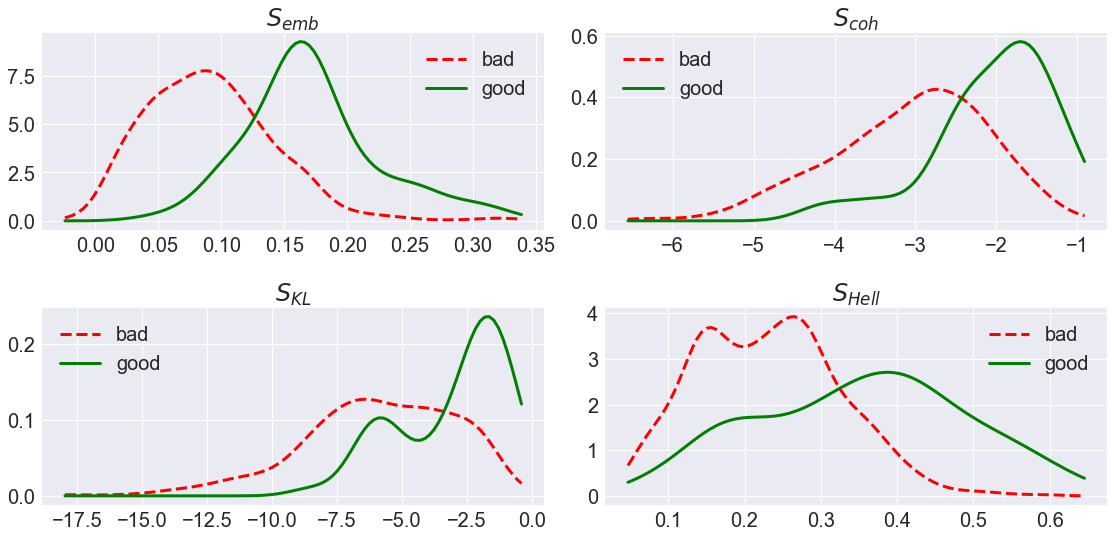
\includegraphics[width=\textwidth]{img/metrics_distr.png}
	\caption{\label{fig:metrics_distr}Вероятностные распределения значений метрик для «хороших»\ и «плохих»\ ребер.}
\end{figure}

В дальнейшем в вычислительных экспериментах используется метрика $\mathrm{S}_{emb}$, так как она показала наилучшую согласованность.

Приведем также качественную иллюстрацию работы метрик. На рисунке \ref{fig:metrics_interpr} приведены 6 пар тем, которые оценивали асессоры в эксперименте. Три из них были оценены как «хорошие», три оставшиеся были оценены как «плохие». 

\begin{figure}[h!]
	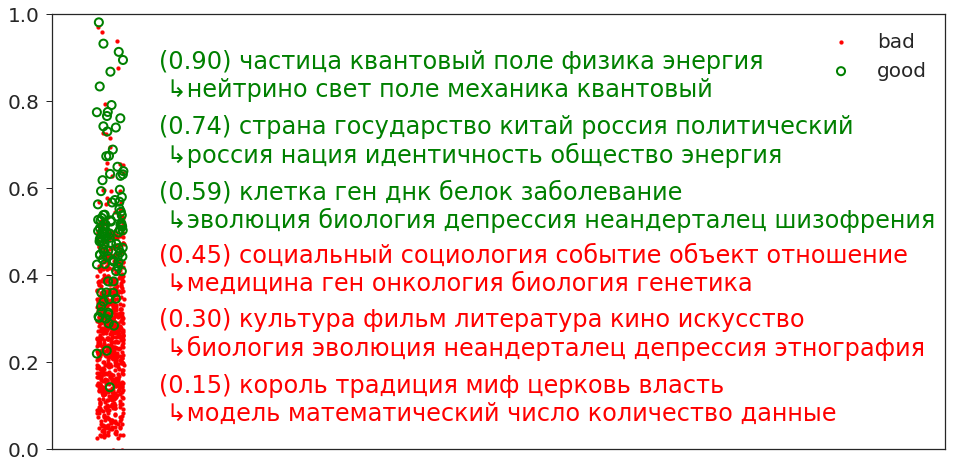
\includegraphics[width=\textwidth]{img/metrics_interpr.png}
	\caption{\label{fig:metrics_interpr}Примеры пар тем из асессорского эксперимента с соответствующими им значениями метрики $\mathrm{S}_{emb}$ и вердиктом асессоров. Каждая тема и подтема представлены своими 5 топ-токенами.}
\end{figure}

Для каждой пары указано соответствующее ей значение метрики $\mathrm{S}_{emb}$. Слева находится распределение всех ребер из асессорского эксперимента. Y-координаты точек соответствуют значениям метрики $\mathrm{S}_{emb}$ для пар тем, а цвета показывают мнение асессоров. Видно, что в эксперименте было гораздо больше пар, оцененных как «плохие», чем тех, которые оценены как «хорошие». Поскольку ожидается, что тематическая иерархия является разреженной (каждая родительская тема имеет только небольшое количество подходящих подтем), это наблюдение соответствует нашим ожиданиям. Из рисунка также ясно, что «плохие» пары имеют более низкое среднее значение метрики, чем «хорошие». Это означает, что метрика $\mathrm{S}_{emb}$ оценивает «хорошие» пары более высокими значениями и, следовательно, коррелирует с мнением асессоров.

\section{Метрики качества тематических иерархий}

Цель состоит в том, чтобы объединить оценки качества ребер в некоторую конструкцию, которая была бы представительной мерой качества для иерархии в целом. Предлагается несколько подходов к этой задаче. Тогда, оценив общее качество связей иерархии с помощью наших метрик и общее качество тем иерархии с помощью метрик для плоских моделей, можно получить представление о качестве иерархии и использовать полученные оценки для сравнения разных моделей.

\subsection{Среднее качество ребер}
В \cite{Mimno2011} качество плоской тематической модели оценивается как среднее качество тем этой модели. Следуя этому же принципу, оценим качество связей иерархии как среднее значение качества ребер. 

Как описано в секции 2.3.2, связи в тематической иерархии задаются вероятностями $p(t|a)$ для пар тем из соседних уровней быть родителем и ребенком. Таким образом, конкретная конфигурация иерархии зависит от порога вероятности, которая является достаточной для включения ребра, соединяющего $t$ и $a$, в иерархию. Поэтому разные пороговые значения приводят к различным значениям среднего качества ребер. Для разных моделей значения $p(t|a)$ могут лежать в разных интервалах. Для того, чтобы сравнивать разные иерархические модели при одинаковых значениях порога, будем здесь и далее использовать нормализованную матрицу $\Psi$:

$$\psi_{ta}^{norm} = \dfrac{\psi_{ta} - \min_t \psi_{ta}}{\max_t \psi_{ta} - \min_t \psi_{ta}}.$$
Тогда $\Psi^{norm} = [\psi_{ta}^{norm}]_{T \times A}$ и для любой модели вероятности имеют значения от 0 до 1.

Недостатком предложенной метрики качества связей иерархии является неинтерпретируемость ее абсолютного значения.

\subsection{Качество ранжирования}

Второй предлагаемый метод оценки качества связей иерархии рассматривает качество ранжирования ребер по значениям вероятностей в матрице $\Psi$. Предположим, что у нас есть несколько уровней иерархии, представляющих собой плоские тематические модели. Если нужно провести фиксированное количество $k$ ребер между темами этих уровней, то естественно выбрать ребра между наиболее связанными с точки зрения человека парами тем. Как показано ранее в секции 3.3, аппроксимацией такого выбора будет набор $k$ ребер с наибольшими значениями метрики $\mathrm{S}_{emb}$. Таким образом, за правильный ответ ранжирования можно взять ранжирование, которое дает метрика и оценить качество ранжирования, которое задает $\Psi$ с помощью принятых метрик качества ранжирования, таких как:

\begin{itemize}
	\item Средняя точность (Average Precision, AP@k) -- описана в \cite{Hang2011}.
	\item Inverse Defect Pairs, IDP@k -- обратное к значению количества пар, которые ранжируются алгоритмом в неправильном порядке.
	\item Normalized Discounted Cumulative Gain, nDCG@k -- описана в \cite{Hang2011}.
\end{itemize}







